\section{Introduction} \label{ch1}

In introducing the analysis of image, videos and computer vision, we first ask ourselves \textbf{"What does it mean to see?"}. An interesting answer was provided by \textbf{David Marr (1982)}, one of the father of visual perception, \textit{"The plain man's answer would be, to know \textbf{what} is \textbf{where} by looking"}. In this sense, his idea was to associate the concept of seeing to the task of \textbf{object detection}, as represented in the following picture:

\begin{figure}[h!]
		\centering
		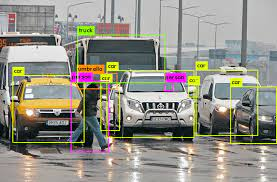
\includegraphics[scale = 0.7]{img/object_detection.jpeg}
        \caption{Object detection problem}
\end{figure}

\subsection{Theory of vision: from Pythagoras to Marr}
The very first theories about vision were:

\begin{itemize}
    \item the \textbf{emission theory}, which thought that the eye was capable of visualizing the objects in the world by using a "fire". An important feature of this theory is that it considered visual perception from a mathematical point of view, and for this reason it was supported by Pythagoras, Euclid and Empedocles;
    \item the \textbf{intromission theory}, which thought that the images came from the objects and entered our eyes. This theory was supported by Democritus, Epicurus and Lucretius;
    \item \textbf{Plato's view}, which can be considered a compromise between the previous theories, in the sense that he believed that the image was captured by the eye using both the "fire" of the eye itself and the "body" of vision of the object;
    \item \textbf{Alhazen's theory}, which was introduced in its \textit{Book of Optics}, representing a new theory of perception and pointing out the weakness of the previous theories;
    \item \textbf{Kepler's modern theory} of retinal images, in which he understood how the images are formed in our eyes.
\end{itemize}

Moreover, along with the different theories we introduced, two fundamental intellectual traditions dominated the biological field of vision:

\begin{itemize}
    \item the \textbf{nativism} (Kant, Cartesio etc..), which thought that there's an infrastructure that allows humans to visualize the objects;
    \item the \textbf{empiricism} (Locke, Hume etc..), which on the other hand thought that humans perceived the external world by learning.
\end{itemize}

Among the Empiricists, a very interesting point of view was provided by \textbf{Helmotz}, who believed in the \textit{vision as an unconscious inference}. More specifically, he thought that visual perception is:

\begin{itemize}
    \item \textit{unconscious}, because we cannot explain why we see or why we recognize things, so we cannot provide a solution to the vision problem since we are not aware of what that is;
    \item characterized by an \textit{inference process}, i.e. that our brain infers the image we see by some other basic features. An example of this inference process is provided by Picture \ref{inference}: in this case we infer the central white triangle from the shapes and the colours of the surrounding objects, even if the triangle is not actually represented.

    \begin{figure}[h!]
		\centering
		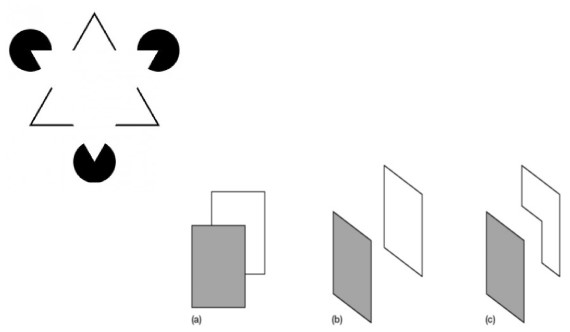
\includegraphics[scale = 1.5]{img/inference.jpg}
		\label{inference}
		\caption{Example of an inference processes}
    \end{figure}

    Another biological example of this inference process is provided by our eye: we know that only the center of the retina (fovea) is composed of perceptors that allow to capture the colours of an object, but the brain collects these samples and forms an image which entirely colored.
    
\end{itemize}

Another important contribution was brought by the \textbf{Gestalt school}, whose goal was to establish some new laws concerning the visual perception. Despite failing in this project, they still managed to introduce some important notions, for example the one of \textit{grouping}, which can be considered nowadays as the \textit{clustering problem}, one of the main issues in Computer Vision.

Finally, \textbf{David Marr} in 1982 provided a new theory about vision, which was based on a mathematical perspective, neuroscience and IT. More specifically, he introduced three levels of understanding the problem of vision :

\begin{itemize}
    \item the \textbf{computational level}, i.e. what does the system do? What problems does it solve or overcome?
    \item the \textbf{algorithmic} or \textbf{representational level}, i.e. how does the system do what it does? What representations does it use and what processes does it employ to build and manipulate the representation? 
    \item the \textbf{implementation} or \textbf{physical level}, i.e. how is the system physically realized? This level addresses the actual implementation of the algorithms.
\end{itemize}

However, we can see that Marr did not consider learning in his theory, and this was pointed out by \textbf{Tomaso Poggio}, who at the contrary believed in learning as the top level of understanding and as the tool which is necessary \textit{"to build intelligent machines that are able to learn to see (and think) without the need to be programmated to do it"}.

\subsection{Computer Vision}
We can describe the goal of Computer Vision as the one of producing a symbolic description of what is being imaged, and for this reason it can be viewed as an inversion of the image process.

\begin{figure}[h!]
		\centering
		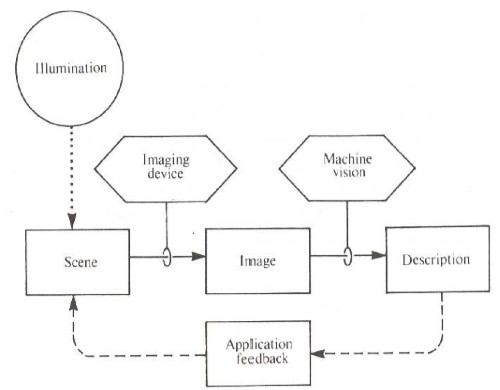
\includegraphics[scale = 1.5]{img/cv.jpg}
\end{figure}

Actually, Computer Vision can be considered as an intersection of many other \textbf{disciplines}, such as:

\begin{itemize}
    \item \textit{Image processing}, which takes as input an image and produces another (possibly) better image. An example of image processing algorithm is image compression;

    \begin{figure}[h!]
		\centering
		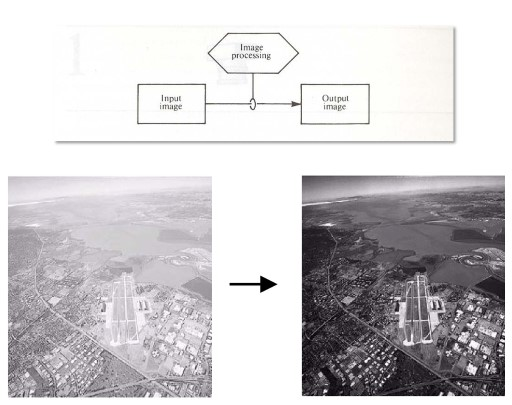
\includegraphics[scale = 1.5]{img/image processing.jpg}
		\caption{Image processing}
    \end{figure}

    \item \textit{Pattern recognition}, which classifies object and detects patterns on them;

    \begin{figure}[H]
		\centering
		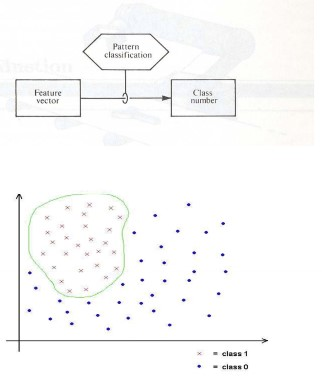
\includegraphics[scale = 1.5]{img/pattern recognition.jpg}
		\caption{Pattern recognition}
    \end{figure}

    \item \textit{Scene analysis}, which provides a high-level symbolic description of the scene;

    \begin{figure}[h!]
		\centering
		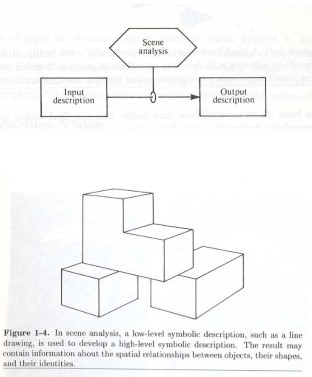
\includegraphics[scale = 1.5]{img/scene analysis.jpg}
		\caption{Scene analysis}
    \end{figure}

    \item \textit{Graphics}, which given a model produces an image (synthesis problem).
\end{itemize}

In general, the historical landmarks in the field of Computer Vision were:

\begin{itemize}
    \item in 1963, Larry Roberts introduced some algorithms, for example edge detection, focusing on the block worlds, i.e. a symplified world in which the objects are represented as blocks;
    \item the \textit{Summer Vision Project} in the summer of 1966, in which the students were asked to produce a visual system for pattern recognition. The task of this project underlines the overall underestimation of the problem of CV;
    \item in the 70's, Marr's idea was to build models and representations of the input image which were more and more abstract. In this sense, the representations were:
    \begin{enumerate}
        \item \textit{Primal sketch}, which is a very primitive representation;
        \item \textit{2-$\frac{1}{2}$D}, which captured the local surface orientation and the discontinuities in depth and in surface orientation;
        \item \textit{3-D model representation}.
    \end{enumerate}
    \begin{figure}[h!]
		\centering
		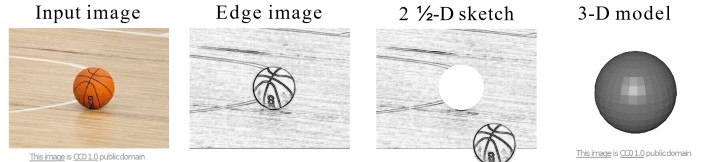
\includegraphics[scale = 1.5]{img/marr.jpg}
    \end{figure}
    \item in the 70's, other 3D representations were introduced, such as the \textit{Generalized Cylinder} or the \textit{Pictorial Structure}, whose goal was to decompose real-world objects and their relations and representing them as graphs;
    \item in 1987 and 1999, Lowe introduced the task of \textit{feature extraction} (SIFT), i.e. he thought that vision can be described as the process of extracting complex features from an image;
    \item the problem of \textit{Image segmentation and clustering}, i.e. partition the image into segments that are coherent from a colour point of view. This problem was the starting point for many other algorithms;
    \item \textit{Face detection}, which led to the first successful algorithm (Viola & Jones, 2001), which was both correct and fast and it was implemented for many years;
    \item \textit{Histogram of Gradients (HoG), 2005}
    \item \textit{Deformable Part Model, 2009}
\end{itemize}

Then, people started building datasets for training Machine Learning algorithms for many CV problems, which pushed the community both to develop more accurate ML algorithms and to have an objective measure of the performances of the CV algorithms. An example of this tendency was the \textit{PASCAL Visual Object Challenge (2006-2012)}, which was an object detection challenge, or the \textit{ImageNET (2009)}, a very large dataset containing various labeled images with a large number of categories (22K categories for 14M images). In 2009, the \textit{Large Scale Visual Recognition Challenge} was instituted, and year after year the performances of the ML algorithms increased, until 2012, when the first Deep Learning approach was introduced, representing a huge change in CV history. 

The idea behind the Deep Learning approach was to get rid of the standard approach, consisting in designing good features and then feed the ML algorithm, and to exploits the learn phase of the algorithms to learn a feature hierarchy. In this sense, each layer of the deep Neural Network extracts features from the output of the previous one, creating a hierarchy and producing a final classifier. Despite being an old idea, Dee Learning was introduced only in 2012 because of the large availability of data and computing power (GPUs).